\documentclass[../PS6_RapportFinal.tex]{subfiles}

\begin{document}
\graphicspath{{img/}{tex/img/}}


\section{Résistance des tubes en flambement}


\begin{figure}[h]
\begin{center}
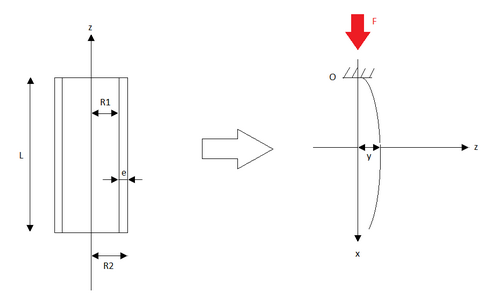
\includegraphics{5_1_resistance_tube.png}
\caption[width=10cm]{Comportement des tubes d'aluminium}
\label{tube_aluminium} % Si vous avez besoin de citer votre figure quelque part dans le texte, dans ce cas, au lieu du numéro de figure, mettez \ref{reference_figure} (i.e. écrire : figure \ref{reference_figure})
\end{center}
\end{figure}

Dans cette annexe, nous allons étudier le flambement du tube lors du plantage dans le compost, et dimensionner celui-ci afin qu'il ne se casse pas.
\\
\\
Théorème du moment à l'équilibre sur $\vec{z}$ :

\[M_{f_{z}}(x) + y(x).F = 0\]

\[\Rightarrow EI.y''(x)+E.y(x) = 0\]

\[\Rightarrow y''(x) + \frac{F}{EI}.y(x) = 0\]

\[\Rightarrow y(x) = Acos(\sqrt{\frac{F}{EI}}x)+Bsin(\sqrt{\frac{F}{EI}}x)\]

Or les conditions limites nous donnent :
\[y(0) = 0 \Rightarrow A = 0\]
\[y(L) = 0 \Rightarrow Bsin(\sqrt{\frac{F}{EI}}L) = 0\]
\[\text{i.e.} \: \exists n \in \mathbb{Z}, \: \sqrt{\frac{F}{EI}}L = n\pi\]
\[\Rightarrow I = \frac{FL^{2}}{En^{2}\pi^{2}}\]
\[\text{or} \: I = \frac{\pi(R_{2}^{4}-R_{1}^{4})}{32}\]
\[\Rightarrow \: I = \frac{\pi(R_{2}^{2}-R_{1}^{2})(R_{2}^{2}+R_{1}^{2})}{32}\]
\[\Rightarrow \: I = \frac{\pi(R_{2}-R_{1})(R_{2}+R_{1})(R_{1}^{2}+2eR_{1}+e^{2}+R_{1}^{2})}{32}\]
\[\Rightarrow \: I = \frac{\pi e(2R_{1}+e)(2R_{1}^{2}+2eR_{1}+e^{2})}{32}\]

Donc :
\[e(2R_{1}+e)(2R_{1}^{2}+2eR_{1}+e^{2}) = \frac{FL^{2}}{En^{2}\pi^{2}}.\frac{32}{\pi}\]
Finalement :
\[e^{4}+4R_{1}e^{3}+6R_{1}^{2}e^{2}+4R_{1}e=\frac{FL^{2}}{En^{2}\pi^{2}}.\frac{32}{\pi}\]

Nous avons effectué l'application numérique avec les valeurs suivantes : $R_{1} = 19 \: \si{\milli\metre} $, $F = 1000 \: \si{\newton}$, $L = 1000 \: \si{\milli\metre}$, $E = 69000 \: \si{\mega\pascal}$, $n = 1$.

Nous obtenons, à l'aide d'un solveur, $e= \num{0.52} \: \si{\milli\metre}$. Il suffit donc de choisir un tube d'épaisseur supérieure à \num{0.52} \si{\milli\metre} afin d'éviter le phénomène de flambement lors du plantage. Nous sommes donc relativement libre quant-au choix du tube. Il est par ailleurs pertinent de préciser que l'étude a été faite sur une seul tube, en exagérant volontairement l'effort de plantage. Il convient donc de diviser ce résultat par le nombre total de pieux, soit 10, afin d'avoir une valeur cohérente avec notre prototype.


\end{document}